\documentclass[]{interact}
\usepackage{epstopdf}% To incorporate .eps illustrations using PDFLaTeX, etc.
\usepackage{subfigure}% Support for small, `sub' figures and tables
%\usepackage[nolists,tablesfirst]{endfloat}% To `separate' figures and tables from text if required

\usepackage{natbib}
\bibliographystyle{chicago}
\setcitestyle{authoryear,open={(},close={)}}
\renewcommand\bibfont{\fontsize{10}{12}\selectfont}% Bibliography support using natbib.sty

\usepackage{hyperref}
\hypersetup{
    colorlinks=true,
    linkcolor=blue,
    filecolor=magenta,
    urlcolor=blue,
    citecolor=blue,
}

\usepackage{titlesec}
\titleformat*{\section}{\Large\bfseries}
\titleformat*{\subsection}{\large\bfseries}

\usepackage{endnotes}
\let\footnote=\endnote
\usepackage{etoolbox}
\patchcmd{\enoteformat}{1.8em}{0pt}{}{}

\theoremstyle{plain}% Theorem-like structures provided by amsthm.sty
\newtheorem{theorem}{Theorem}[section]
\newtheorem{lemma}[theorem]{Lemma}
\newtheorem{corollary}[theorem]{Corollary}
\newtheorem{proposition}[theorem]{Proposition}

\theoremstyle{definition}
\newtheorem{definition}[theorem]{Definition}
\newtheorem{example}[theorem]{Example}

\theoremstyle{remark}
\newtheorem{remark}{Remark}
\newtheorem{notation}{Notation}
\usepackage{csquotes}

\usepackage{tabularx}
\usepackage{booktabs,caption}
\usepackage{threeparttable}

\usepackage{lscape}
%%%%%%%%%%%%%%%%%%%%%%%%%%%%%%%%%%%%%%%%%%%%%%%%%%

\begin{document}

\articletype{DRAFT MANUSCRIPT}

\title{Replication Survey}

\author{
\name{Peter Kedron\textsuperscript{a,b}\thanks{CONTACT Peter Kedron. Email: peterkedron@ucsb.edu}, Joseph Holler\textsuperscript{c}, and Sarah Bardin\textsuperscript{b,d}}
\affil{\textsuperscript{a} Department of Geography, University of California Santa Barbara, Santa Barbara, California, USA; \textsuperscript{b}School of Geographical Sciences and Urban Planning, Arizona State University, Tempe, Arizona, USA; \textsuperscript{c}Department of Geography, Middlebury College, Middlebury, Vermont, USA
\textsuperscript{d}Spatial Analysis Research Center (SPARC), Arizona State University, Tempe, Arizona, USA; }
}

\maketitle

\begin{abstract}
Write Abstract

\end{abstract}

\begin{keywords}
Reproducible Research, Epistemology, Geographic Research Methods
\end{keywords}

%%%%%%%%%%%%%%%%%%%%%%%%%%%%%%%%%%%%%%%%%%%%%%%%%%
\newpage
\section*{Introduction}
Replications confront existing explanations with new evidence by retesting prior claims using new data and similar research procedures.
Replications can be designed to serve different epistemic functions and to test several forms of validity.
Attempts to reproduce prior research may also test the validity of a study, but do so using the same data and the same, or very similar, analyses. 
Contrasted with a replication attempt, the central focus of a reproduction attempt is the verification of claims through the examination of how a study was conducted and whether the design and execution of that study supports the results presented.
While the results of a reproduction or replication do not provide conclusive evidence for or against a claim, those that produce outcomes consistent with prior studies typically increase confidence in a claim and the theories upon which it is based \citep{earp2015, nichols2021}. 
When prior results cannot be recreated, there is reason to question the data and methods used by the prior study, the claims made by the prior study, and perhaps even the current theoretical understanding of the geographic phenomena \citep{christensen2019, NASEM2019}.

While the number of reproduction and replication studies undertaken in the social and behavioral sciences continues to rise, such studies have not yet become commonplace in geography.
The majority of recent research in the geographic literature on the subject has focused on reproduction over replication, and has emphasized the computational reproducibility of geographic research ahead of other dimensions.
For example, an ongoing reproducibility initiative supported by the Association of Geographic Information Laboratories in Europe attempts to reproduce the computational results of submissions to their annual meeting and reports on the accessibility of related data, code, and computational environment \citep{nust2018, ostermann2021}.
A series of reproduction studies led by Kedron and Holler \citep{Kedron2023Beyond, Kedron_Holler_Bardin_Hilgendorf_2022} advance this stream of work by introducing selected variations into the reproduction process to test the sensitivity of results to conceptual and methodological perturbations. 
However, those studies also largely focus on testing the conclusion validity of past studies through computational reproduction. 

The small number of published studies that have attempted to replicate geographic research suggest that many studies cannot be fully replicated \citep[e.g.,][]{Kedron2022dimaggio, paez2022reproducibility}, or are simply missing components needed to attempt a replication \citep{konkol2019, ostermann2017}.
More often the literature on the replication of geographic research turns to the question of if and when it is reasonable to expect the findings and claims of a prior study to be replicable \citep{kedron2021GA, kedron2022replication, goodchild2021replication, sui2021reproducibility}. 
Place-to-place variations in phenomena, and the processes that produce those variations, are one of the defining features of geographic research and a central tenet of many of its research traditions.
With these intellectual foundations, it remains unclear how current geographic researchers view replication and its role in the knowledge accumulation process.
There is similarly limited empirical evidence available about the factors that motivate or discourage geographic researchers from pursuing replications. 

To address this gap in our collective knowledge, we surveyed geographic researchers about their understanding of replicability, beliefs about what factors affect the chances of replicating a study, motivations to attempt replication studies, and experiences conducting replications.
We are aware of only a handful of similar published surveys within the geographic literature \citep{balz2020reproducibility, konkol2019, ostermann2017, kedron2023survey}.
However, these surveys typically focus on the quantitative and computational intensive forms of geographic research, primarily assess the availability of research artifacts (e.g., data and code), and address reproducibility rather than replicability. 
In all but one instance, these surveys also rely on convenience samples drawn from specialist conferences or non-representative subsets of the geographic research community. 
In contrast, to support generalization, we designed a sampling frame to capture researchers from across disciplinary subfields and methodological approaches, and draw survey participants from that frame using a probability sampling scheme.

In the remainder of this paper, we first briefly present the epistemic roles of replication in the context of geographic research.
We then detail the design of our survey, sampling strategy, and analytical approach before presenting our results. 
We conclude with a discussion of the implications and limitations of our work. 


%%%%%%%%%%%%%%%%%%%%%%%%%%%%%%%%%%%%%%%%%%%%%%%%%%
\section*{Replication and the Evaluation of Prior Claims}
Replications structure the iterative development of theory by confronting claims with new evidence.
Broadly defined, a replication is any study that has at least one outcome that would be considered diagnostic evidence of the validity of a claim made in prior research \citep{nosek2020}.
No single study provides evidence about all conditions that could affect a claim, because individual studies are performed by particular researchers using particular methods to draw and analyze data from particular settings. 
Until a claim is tested through replication, our expectation of whether it will hold under new conditions relies on the theory used to structure the original investigation or on a speculative assumption of generalizability.
Replications empirically test the validity and reliability of the claims made in a study by selectively altering different aspects of the initial work and repeating the study \citep{schmidt2009, gomez2010replications, radder2003, radder2012}.  
By altering different aspects of a study across a series of replications, researchers can collectively and progressively test claims across a widening set of conditions and use that information to revise theory.

The type of check a replication provides depends on which aspects of a study are changed and in what combination. 
Researchers pursuing a replication will collect new data, but will also change the materials and procedures used in the replication, the measurement of variables, the location of the replication, and/or the population being studied \citep{hendrick1990, schmidt2009, gomez2010replications}. 
Replication studies are often classified as either direct or conceptual depending on which of these aspects a researcher is changing and the epistemological objective they are pursuing \citep[see][]{sargent1981repeatability, schmidt2009, plesser2018reproducibility}.

Direct replications make limited changes to an initial study in order to verify the claims of the study by testing for conclusion, construct, and internal validity. 
If a researcher attempting a replication keeps all aspects of a study the same, but collects new data, then the replication is designed to assess conclusion validity.
As long as the population being studied remains stable between the two studies, the replication will control for sampling error and will provide evidence as to whether the prior results were the product of chance variation. 
Alternatively, if a researcher changes how a key construct is measured and also holds all other aspects of a study constant, then the replication can test construct validity.
Consistently observing a relationship across well-established measures of a concept or phenomenon may raise researcher confidence that the operationalization used in the original study did not bias the result or affect the claims made. 
Finally, if the materials and procedures (e.g., data collection device, analyses) used in a replication differ from a prior study, then the replication assesses whether these factors affected the original results, thereby testing the internal validity of the prior work. 

In conceptual replications, changes are made to the population or location being studied in order to test external validity and whether the claims made in a study generalize to new populations and contexts. 
In geographic research, a conceptual replication could involve changing the location of a study from one city to another or from one ecosystem to another. 
Alternatively, a researcher could conduct a conceptual replication of a study by examining the same location across different time periods, for instance, before and after migration is thought to have changed the population within that area. 
Conceptual replications provide evidence that can be used to assess the hypotheses and theories that underlie a prior study in new situations \citep{schmidt2009}.
However, conceptual replications do not necessarily provide evidence that can be used to adjust confidence in a claim made in an initial study \citep{nosek2020}.
For example, it is not necessarily the case that observing evidence in one location that contradicts a prior study's claim based on a different location should reduce a researcher's confidence in the prior claim.

As tests of generalizability and external validity, conceptual replications play an important role in the development of theory \citep{earp2015, haig2022, irvine2021}.
When a theory is early in its development, it is often unclear whether a researcher should expect the predictions of that theory to hold in new populations, locations, and times.
This is the case because new theories commonly lack a well developed set of conditional statements identifying for whom, where, and/or when their explanations and predictions should hold. 
Without these statements, it remains possible that the predictions of the theory will generalize across a large set of contexts. 
In other words, a lack of evidence causes uncertainty about the explanatory range of the theory.
In this situation, conceptual replications act as empirical tests of the external validity of a theory. 
Conceptual replications provide evidence to inform the addition and revision of conditional statements that identify for whom, where, and/or when the theory is expected to provide meaningful predictions.
As the conditions required for a claim to replicate are incorporated into the theory, the theory matures and the situations in which the prediction of the theory are expected to hold becomes clearer.

%%%%%%%%%%%%%%%%%%%%%%%%
\subsection*{The Replicability of Geographic Research}
Geographers have arguably never formally and explicitly held an extended discussion of the role of replication in the discipline.
However, replication is implicitly at the center of the discipline's nomothetic-ideographic debate \citep{kedron2022replication, sui2021reproducibility} and ongoing discussions about how to construct explanations of the physical and human processes that shape the world \citep[see][]{harvey1969, inkpen2013science, miller2015data, sayer1992method, yeung2019rethinking, yeung2023theory}. 
Within this literature, discussions of replication typically pivot on the expected variability of processes across locations, whether replications can inform theory development and, as a practical matter, the ability to control factors that may affect the outcome of a study. 

The first point raised in most discussions of replication in geography is that places are unavoidably different from one another \citep[see][]{goodchild2021Annals, goodchild2022reproducibility, Wainwright2021}.
Researchers involved in these discussions often invoke \cite{anselin1989special} second law of geography which notes that geographic features exhibit uncontrolled variability over space. 
This principle implies that researchers can expect to observe differences between places, which may contribute to an inability to replicate prior findings from one place in another.
Geographic variation essentially poses an identification problem for those interpreting the results of a replication, because it is not clear whether the same research outcome (e.g., parameter estimates) observed in different locations is or is not determined by the same processes.  
In some instances, commentary about differences between places are combined  with discussions of role of researcher position and perspective in the research process \citep{Peet1999, simandan2019revisiting}. 
Discussions of replication developed from this perspective often suggest that the role replication can play in geography is limited, because research is an interpretive process dependent on the unique perspective of a researcher who is analyzing data drawn from different or unique places \citep{Wainwright2021}. 

Arguments about geographic variation can be pushed further and linked to the principle of flux \citep{marcovich1967}. 
This alternative argument suggests that, on the one hand, phenomena studied in a place cannot be encountered twice, and, on the other hand, that places are defined not by the stability of their features but by their continual renewal through processes that create change in those same features. 
The two alternative readings of this principle have very different implications for the prospect of replicating geographic research.
Under the first simpler reading, change is constant and a researcher should not expect to find the same arrangement of features at different times in the same location.
In this situation, an inability to replicate a finding would not be surprising and explanations would be localized. 
Under the second reading, geographic features are continually changing but are structured by processes that may, or may not, be consistent across time and space. 
In this situation, findings may be expected to replicate within a range of uncertainty, and attempting replications can give insights into the stability of processes across locations. 

Understanding places as defined by processes that potentially differ across locations aligns with the argument that geography is well-suited to the development of empirically grounded middle-range theory \citep{miller2015data}.
The aim of middle-range theory is not to develop overarching explanations or essential features of processes, but rather to offer provisional explanations of identifiable phenomena, which can be tested and used to slowly develop more general but bounded explanations \citep{merton1968social}.
As \cite{harvey1969} notes, geographers often elaborate the theories of other disciplines by linking them with spatial explanations of form and process.
\cite{turner1989, turner2002} argues this synthesis approach gives geography the capability to generate and refine the text of theories and establish their spatial domain by examining phenomena empirically within a web of complex processes that interact within and between locations. 
In this way, replications can give insight into when, where, and why an explanation does not hold \citep{zhang_wolf_2023}.
Similarly, \cite{sayer1992method} distinguishes between intensive research in which synthesis is used to identify how processes work in a particular case of location, and extensive research in which synthesis extends across cases or locations to identify how widely a process holds. 
In intensive research, replication attempts that change the data collected from a location can be used to corroborate the explanation of a process.
In extensive research, replication data is gathered from new contexts to establish the coverage of an explanation. 
In either case, that accumulation of empirical evidence through replication can be used to refine and adjust theory.

Finally, discussions of replication in the literature also frequently point out that many of the phenomena geographers study not only vary across locations but are difficult or impossible to control \citep[see][]{sayer1992method, kedron2021GA, waters2021motivations}. 
In practice, geographers often lack the ability to control where data is collected, which populations are included or excluded in a study, how variables are measured, and the materials and procedures used when attempting a replication.
This lack of control makes it difficult to execute replications that isolate the influence of any particular factor, which makes it unclear what lessons should be learned from a replication attempt and what epistemological function that attempt may be serving. 
Moreover, it is also often unclear which factors should be accounted for when studying a particular location.
As \cite{goodchild2021replication} suggest, even when some level of control can be exerted on a process, it will remain difficult to exclude the variable effects of context from studies that are incompletely identified in the presence of spatial heterogeneity.
While these factors make replication practically challenging in some forms of geographic research, they do not themselves eliminate the potential usefulness of the practice in selected cases. 

Geography as a discipline is presently defined by its topical, epistemological, and methodological diversity. 
While replication has been an implicit part of many discussions of the development of knowledge in the discipline, it remains unclear exactly how the practice is understood and applied by researchers within those different traditions.
Moreover, to date there has been no empirical measure of how often researchers across the discipline attempt to replicate research, what motivates them to pursue or not pursue replications, and how they would interpret the findings of such studies. 
In fact, we expect that many geographic researchers would disagree with the conception and presentation of replication presented above. 
However, until researcher conceptions and practices of replication are systematically assessed, conversations about the role of replication in the discipline can only progress so far.


%%%%%%%%%%%%%%%%%%%%%%%%%%%%%%%%%%%%%%%%%%%%%%%%%%
\section*{Data and Methods}
Complete documentation of the procedures, survey instrument, and other materials used in this study are available through the Survey of Researcher Perceptions of Replication in Geography project (\citet{Kedron_Holler_Bardin_Hilgendorf_2022} - \url{https://osf.io/x6qrk/}).
This OSF project connects to a GitHub repository which hosts the anonymized dataset and code used to create all results and supplemental materials along with a complete history of their development. 
All of the results presented in this paper can be independently reproduced using the materials in that repository.
Before the start of data collection, we preregistered an analysis plan for the survey with OSF Registries (\citet{Kedron_RPl_Survey_PAP} - \url{https://osf.io/a4nwg}). 
The survey was conducted under the approval and supervision of the Arizona State Institutional Review Board - \textit{STUDY00014232}.

%%%%%%%%%%%%%%%%%%%%%%%%
\subsection*{Sampling Frame}
Our target population of interest is researchers who have recently published in the field of geography. 
We followed a 4-step procedure to create a sampling frame for our survey that captures this diverse population of researchers. First, beginning at the publication level, we identified journals indexed as either geography or physical geography by the \href{https://access.clarivate.com/}{Web of Science's Journal Citation Reports} that also had a 5-year impact factor greater than 1.5.
From those journals, we created a database of all articles published between 2017 and 2021.  
Second, we used Arizona State University's institutional subscription to the \href{https://www.scopus.com/home.uri}{Scopus Database} to extract journal information (e.g., subject area, ranking), article information (e.g., abstract, citation counts), and author information (e.g., corresponding status, email) for each publication. 
Because our intention was to capture individuals actively publishing new geographic research, we retained publications indexed by Scopus as \textit{document type = ``Article''} and removed all other publication types (e.g., editorials, book reviews) from our article database. 
We also removed articles with missing authorship information. 

Third, moving to the researcher level, we created a list of researchers and their published articles, focusing on corresponding authors for two reasons.
(1) Corresponding authorship is one indicator of the level of involvement an individual had in a given work. 
While imperfect, it was the best available indicator in the Scopus database as across journals there is no commonly adopted policy for declarations of author work (e.g., CRediT Statements).
(2) Scopus maintains email contact information for all corresponding authors, which gave us a means of contacting researchers in our sampling frame.
Scopus also maintains a unique identifier for each author (author-id) across time, which allowed us to identify authors across publications. 

Fourth, we constructed a sampling frame of unique researchers and their most recent email contact information. 
We determined uniqueness by grouping researchers by their author-id, and we determined the most recent contact information by selecting records associated with the most recent year of publication. 
For 383 researchers who had two or more distinct emails in the latest year of publication, we removed non-institutional personal email addresses and then selected one of the remaining institutional email addresses.

Applying these criteria yielded a sampling frame of 29,828 researchers. 
On average, these authors published 2.7 articles in geography journals meeting our criteria between 2017 and 2021. 
Roughly one-third (33.0\%) were most recently a corresponding author for an article published in a general geography journal. 
A similar proportion (32.0\%) were most recently a corresponding author for an article published in an earth sciences journal, and smaller proportions had published in the social sciences and cultural geography (20.0\% and 16.0\%, respectively).

\subsection*{Survey Instrument}
The survey first established eligibility based on age and geographic research activity in the past five years and asked researchers to report their primary subfield and methodology.
We asked each participant to assess their familiarity with the term ``replicability'' and to provide their own definition. 
We then provided a definition based on \citet{nosek2020} to establish a common understanding of replicability for the remainder of the survey.
Specifically, replication was defined as,

\begin{displayquote}
    ``A \textbf{Replication} is any study that seeks to evaluate a claim of a prior study using similar procedures and new data. A claim made in a prior study have been replicated when the replication produces outcomes that are consistent with the prior claim and increase confidence in that claim."
\end{displayquote}

\noindent Remaining questions assessed the epistemological purpose of a replication (5 questions), what portion of the geographic literature has/could/should be replicated (3 questions), and factors that impact the chances of successfully replicating a study (18 questions) or the decision to attempt a replication (13 questions).
For researchers who reported attempting reproductions, we asked them to elaborate on their motivations and outcomes (9 questions).

We developed the survey questions following a review of prior reproducibility surveys \citep[e.g.,][]{fanelli2009many,baker20161, konkol2019} and our own reading of recurring issues in the reproducibility and replicability literature. 
We pre-tested the survey instrument with \textit{n}=15 graduate students and geography faculty with differing levels of experience, topical focus, and methodological background. 
After pilot testing, we removed these individuals from our sampling frame to ensure they would not be included in our final sample.

%%%%%%%%%%%%%%%%%%%%%%%%
\subsection*{Data Collection}
We used a digital form of the Tailored Design Method \citep{dillman2014internet} to survey geographic researchers between Oct 3 and Oct 27, 2022.
A simple random sample of 2,000 researchers was drawn without replacement from our sampling frame, and those researchers were invited via email to participate in the online survey. 
Researchers received their initial invitation on Oct 3, 2022. 
Two reminder emails were sent on Oct 13 and Oct 20, 2022 to researchers that had not yet completed the survey.

The online survey was administered through \href{https://www.qualtrics.com/}{Qualtrics}. 
Participation in the survey was entirely voluntary. 
Each researcher that opted to participate in the survey was provided with IRB-approved consent documentation and linked to the internet survey instrument. 
Participants were also given the option to provide an email address for eligibility for one of three  prizes of 90 US\$, selected randomly after the data collection period.
Participating researchers had the option to exit and re-enter the survey and were also able to review and change their answers using a back button as they progressed through the survey.
At the end of the data collection period, responses were checked for completeness and coded using the reporting standards of the American Association For Public Opinion Research \citep{aaporstandards}.
Responses were downloaded from Qualtrics, anonymized, and stored in a public de-identified database in the research compendium.

%%%%%%%%%%%%%%%%%%%%%%%%
\subsection*{Analytical Approach}

We conducted two analyses of the survey responses.
First, we analyzed researcher perspectives on replicability by coding and calculating summary variables and statistics for three themes: how geographic researchers define replicability, factors researchers believe affect the decision to attempt to replicate a study, and factors researchers believe affect the chances of successfully replicating a study.
Second, we analyzed the experiences of researchers attempting to replicate prior studies using statistical summaries of participant motivations, research practices, and ability to produce results consistent with prior studies.
For both analyses, we produced and analyzed descriptive statistical summaries of participant responses to Likert scale questions cross-tabulated by disciplinary subfield and methodological approach.
For free-form text responses we coded responses and selected illustrative examples for inclusion. 

For free-form text definitions of ``replicability'' we coded participant responses using two procedures. 
First, we measured the similarity of each provided definition to the definition adopted by the \citet{NASEM2019}. 
The NASEM defines replicable research as having three characteristics --- new data, same procedure, and same or similar results.
To make this comparison, two of the authors independently coded each respondent definition for the presence/absence of each of these three characteristics.
Disagreements in the assignment of codes were resolved through discussion between the three authors.
We created an aggregate measure of definition similarity for the final coded response for each participant by counting the presence of each NASEM definition characteristic, resulting in a measure with the domain [0, 3].

Second, we coded each definition to identify mentions of: (i) internal validity assessment, (ii) external validity assessment, (iii) the significance of spatial or temporal context, (iv) epistemological necessity, and (v) adherence to open science practice.
We derived this coding from common themes in the responses and our own reading of the replicability literature.
As above, each definition was independently coded by each author before code assignments across authors were compared with disagreements resolved through discussion.
Our first set of analyses examined the full set of survey responses, while our second set of analyses were restricted to the 84 participants that reported attempting a replication study in the past two years.

%%%%%%%%%%%%%%%%%%%%%%%%%%%%%%%%%%%%%%%%%%%%%%%%%%
\section*{Results}
A total of \textit{n}=283 of the authors we contacted completed the online survey with information sufficient for analysis. 
The contact rate for the survey was 18.8 percent, the response rate was 14.1 percent, yielding a cooperation rate of 74.4 percent. 
The refusal rate was 4.8 percent\endnote{All outcome rates are reported using \citet{aaporstandards} standards. 
The outcome rates used were - response rate 2, cooperation rate 2, refusal rate 1, and contact rate 1.}.
Respondents were predominantly male (65.1\%) and between the ages of 35 and 55 (62.4\%). 
The majority of respondents were also academics, but were well-balanced across career levels as no one category made up more that 30 percent of the sample.
Respondents were similarly balanced across disciplinary subfields but did contain a greater number of physical geographers  - human geography (26.8\%), physical geography (39.9\%), nature and society (14.8\%), geographic methods and GIScience (17.3\%). 
Different methodological approaches were well-represented by respondents in the sample with qualitative researchers making up the smallest sub-group  - quantitative (47.3\%), qualitative (16.3\%), and mixed-methods (36.0\%).

%%%%%%%%%%%%%%%%%%%%%%%%
\subsection*{Researcher Definitions of Replication and its Epistemic Functions}
Geographic researchers are thinking about replicability and link the act of replicating a study to a number of different epistemological functions. 
A majority of respondents reported thinking about replicability (74\%), talking with colleagues about replicability (65\%), and considering replicability when undertaking peer-review (59\%) during the past two years. 
Specifically, respondents believe that replication studies can assess whether the claims of that study will hold in new locations (67\%) or new populations (63\%) (Figure \ref{fig:Q7-Epistemology}).
Respondents also believe that replication studies can be used to investigate and assess whether the variables used in prior studies reflect the concepts that they were intended to represent (76\%) and whether prior findings resulted from chance variation (66\%).
While respondents clearly linked replication to epistemological functions, across all functions they were more likely to agree than to strongly agree that replications could serve these purposes.
Respondents that identified as human geographers or as studying nature and society were less likely to agree that replications could be used to achieve these goals when compared to those working in other subfields. 
For example, 87 percent of respondents specializing in GIScience and methods believe replications could be used to assess whether a claim was the product of chance, compared to just 57 percent of human and nature-society researchers.

\begin{center}
\textbf{Insert Figure \ref{fig:Q7-Epistemology} About Here}
\end{center}

While respondents largely agree that replication has some epistemological role to play in the geographic research process, many respondents did not explicitly include these same concepts in their definitions of replicability.
A total of 253 of our respondents provided an interpretable definition of replicability, but only 68 of those definitions (26\%) referenced some form of epistemological function. 
Using replication to externally validate the claims of a study was identified by 49 respondents (19\%).
No other epistemological function was mentioned by more than 13 respondents (5\%).  
In contrast, 123 respondents (48\%) reported that replications could be used to assess or improve how well a prior study conforms to the principles of open science (e.g., sharing data and procedures).

Within the limited subset of respondents that explicitly discussed epistemology in their definitions, a small number of researchers carefully articulated connections between the assessment of external validity and the investigation and influence of geographic and temporal context. For example, one participant defined replicability as, 

\begin{displayquote}
``the degree to which a study could be conducted in the same way again, at a different point in time and by other people. Good replicability necessitates that study sites, methods and materials are described in adequate detail. But then there's the question of what replicability means in observational studies where the whole setting of the study changes in time (e.g. forest succession in study sites) so that the study cannot be repeated in the same way in the same area again. Also, there's a difference between replicability of a study and replicability of results. A replicable study does not automatically yield replicable results."
\end{displayquote}

\noindent More often, respondents simply labelled validity checks as the purpose of a replication. One such researcher defined replicability as, ``The ability to reproduce a study using the same or similar research design to test both its internal and external validity." 

A number of respondents specializing in qualitative research provided definitions that questioned, or even rejected, the role of replication in their subfield. 
One qualitative researcher articulates this position by defining replicability as, 

\begin{displayquote}
    ``the claim that empirical research of a study can be repeated in the same way as it was done in the study. However, this is not exactly possible in qualitative research, as data collection is always a co-construction between all persons involved in the data collection. Transferred to qualitative research, this means for me rather that one would use the same questions, analyse the data with the same methods, etc. The fact that the results are not necessarily the same is not a weakness, but rather to be expected, since our knowledge is always embedded and co-constructed." 
\end{displayquote}

Rather than focusing on these larger concepts, most respondents used their definitions to present the criteria that identify a study as a replication.
On average, respondents provided definitions that included 1.2 of the three characteristics of the replicability definitions adopted by the NASEM.
Comparing the similarity of results between studies (65\%) and using the same method across studies (56\%) were the characteristics of replicability most frequently identified by respondents.
Less than a quarter of respondents explicitly included use of the collection of new data (12\%) in their definitions.
Only seven percent of respondent definitions included all three characteristics identified by the NASEM.
A representative definition provided by one respondent identified replicability as, ``That another researcher can get the same results as you by using the same methodological approach."
The pattern of similarity to the NASEM definition and each of its components was consistent across subfields and methodological approaches, with a slightly greater emphasis placed on methodological consistency by quantitative and geographic methods and GIS researchers.

%%%%%%%%%%%%%%%%%%%%%%%%
\subsection*{Factors Affecting the Chances of Replicating a Prior Study}
Overall, respondents believe that the majority of research in the discipline has not been independently replicated and appear to be uncertain about what proportion of the literature could or should be replicated (Figure \ref{fig:Q12-HCS}). 
On average, respondents estimated that 25 percent of recent studies in their sub-field have be replicated. 
However, the distribution of these responses is strongly right skewed.
In fact, 47 percent of respondents estimated that less than 10 percent of recent studies have been replicated.
It is similarly unclear if respondents believe recent geographic research could or should be replicated.
On average, respondents estimated that approximately half of studies `could be replicated' (55.0\%) or `should be replicated' (55.9\%). 
However, the distribution of responses to both questions are relatively flat across the range of possible values and highly variable (\textit{$sd_{could}=24.3\%$}, \textit{$sd_{should}=27.7\%$}), which suggests 
respondents were uncertain whether it was possible or valuable to replicate recent research.  
This pattern of response was consistent across respondents that self-identified as working in different subfields and methodological approaches.

\begin{center}
\textbf{Insert Figure \ref{fig:Q12-HCS} About Here}
\end{center}

Respondents identified a range of study characteristics that might impact the chances of an independent researcher replicating the claims of a prior study (Figure \ref{fig:Q8-10-Chances}a).
A majority of respondents identified the transparency and availability of the components of a study as affecting the odds of replication. 
Poor documentation of the original study (75\%) and the use of restricted access data (66\%) were seen by the greatest number of respondents as decreasing the odds of being able to replicate a prior result. 
Some respondents identified the inclusion of multiple sites in a study as increasing the chances of an independent replication of the findings of that study (39\%), but not in great enough numbers to constitute a majority. 

Respondents were generally uncertain or pessimistic about how the characteristics of the researchers and teams of prior studies would change the chances of replicating the studies. 
A majority of respondents (51\%) indicated that a large research team working on the prior study would have no effect on the chances of an independent researcher replicating that work. 
The remaining respondents were nearly evenly split as to whether a large team would increase or decrease the chances of replicating that study. 
More respondents believed that reliance on the unique expertise (48\%) or unique position(s) (53\%) of the researcher(s)  conducting a study would decrease, rather than increase, the chances of replicating the claims of a study.
In both cases, 24 percent of respondents reported that they did not believe either factor would impact the odds of replicating a prior result.

Respondents were also divided about the extent to which the approach adopted in the prior study would affect the chances of replicating that study. 
Respondents were nearly evenly split as to whether the number of hypotheses tested by a study, and whether that study used qualitative or mixed methods, would increase or decrease an independent researcher's chances of finding results that supported the claims of the prior study.
About a quarter of respondents said that use of a mixed methods approach or the testing of multiple hypotheses had no effect on the chances of replication.
In contrast, a large majority (80\%) of respondents identified the use of quantitative methods in a prior study as increasing the chances of replicating that study. 
This result matches the association observed in respondent definitions of replication, which ties replication to positivist science and quantitative approaches to knowledge creation.   

\begin{center}
\textbf{Insert Figure \ref{fig:Q8-10-Chances} About Here}
\end{center}

There was less agreement among respondents about whether different characteristics of a phenomenon would impact the chances of replicating the claims made by a prior study of that phenomenon (Figure \ref{fig:Q8-10-Chances}b). 
For all six of the characteristics we examined, at least 12 percent of respondents replied that those factors would have no effect on the chances of replicating a prior study.
Numerous respondents also replied that they simply did not know whether a characteristic would impact the chances of replicating a study, resulting in a total of 18 to 42 percent of respondents reporting neutral or uncertain opinions about the characteristics of a phenomena and the replicability of research about it.
For example, 20 percent of respondents said they did not know whether a phenomenon being spatially dependent with itself would affect the chances of replicating a prior study, and an additional 15 percent of respondents said spatial dependence would have no effect on replication. 
Respondents also favored `somewhat likely' responses over stronger `very likely' responses across all characteristics, which further suggests that absence of a clear consensus or understanding of how these factors relate to and impact replication.

Even with this uncertainty, respondents were clearly more concerned about the impact of spatial dependence and place than about spatial variability.
41 percent of respondents reported that the presence of spatial dependence in a phenomena was likely to decrease the chances of replicating a prior study.
A stronger majority of 59 percent reported that phenomena linked to place-based local conditions would decrease the chances of replication.
Meanwhile, respondents were split about whether spatially variable phenomena would increase or decrease the chances of replication.

Respondents were more decisive about replication issues due to an inability to measure or manipulate phenomena than about the presence of multiple possible explanations.
A majority of respondents identified the inability to directly measure a phenomenon (61.5\%) as reducing the chances of replicating a prior study.
A large number of respondents (42\%) were either neutral or undecided on whether the inability to experimentally manipulate a phenomena impacts the replicability of studies about it, with a majority of the remaining respondents agreeing that this inability would decrease the chances of replication. 
An equally large number of respondents were neutral or undecided on whether the presence of a large number of plausible explanations for a phenomena would impact the chances of replicating studies about it, with no clear trend.

%%%%%%%%%%%%%%%%%%%%%%%%
\subsection*{Factors that Affect the Decision to Attempt Replications}
Several factors related to academic incentives and the availability of prior study research artifacts appear to affect whether researchers decide to attempt to replicate recent geographic research, with relatively less concern about the characteristics of prior studies (Figure \ref{fig:Q15-DecisionFactors}).

Geographic researchers identified current academic incentives as the factor most frequently impacting the decision to attempt a replication study. 
A majority of respondents identified the pressure to publish original research (66\%) and the lack of funding for replication studies (59\%) as frequently or always impacting the decision to attempt a replication.
Respondents also believed that the perception of replications as low value work (55\%) that was often difficult to publish (51\%) also impacted decision making.  
Contrary to some narratives in the replication literature, the desire to identify fabricated data or results was not seen as a determining factor in the decision to attempt a replication. 
However, this finding should be interpreted with caution as a third of respondents indicated that they did not know whether potential fabrication influenced researcher decision making.  

\begin{center}
\textbf{Insert Figure \ref{fig:Q15-DecisionFactors} About Here}
\end{center}

Respondents also identified the availability of research artifacts as important to the decision to attempt a replication study.
Respondents believe that difficulty accessing and recreating data (54\%) frequently or always affects the replication decision.
Similarly, respondents (45\%) identified the accessibility of procedural and methodological information as a influential factor. 
The challenge of recreating the methods of a prior study elicited a similar response (41\%).

No characteristics of the original study, or the potential replication attempt, were identified by a majority of researchers as frequently or always impacting the replication decision. 
However, some respondents did identify inexperience conducting replication studies (37\%) and potential geographic variation in the phenomena being investigated (33\%) as always or frequently influencing decisions to attempt replications. 
Moreover, many respondents also saw these factors as occasionally affecting the decision to attempt a replication.
Few respondents see a low chance of successfully replicating a study as a deterrent to attempting a replication, but it is unclear whether this result is driven by a belief in the value of null replication results or the belief that replications have high chances of success.
Finally, respondents did not identify ethical concerns as a factor affecting the decision to attempt a replication study. 
However, these results should also be interpreted in the context of the different levels of uncertainty respondents expressed for each question. 
More than 15 percent of respondents replied that they did not know whether geographic variation, inexperience with replication, or ethical concerns would affect a researcher's decision to attempt a replication. 

Respondents also qualitatively identified a number of factors that were omitted from our survey instrument as important when deciding whether to attempt a replication of a geographic study. 
These factors include practical issues, such as the difficulty identifying and accessing new field sites where data would be collected during a replication attempt, the costs of conducting a replication, and the time needed to obtain institutional ethics approvals.
Respondents also identified uncertainty about how to compare the results of a replication attempt to the original as important when deciding to undertake a replication attempt. 
For example, one respondent noted that. ``Given expected spatial variation, it can be difficult to arrive at a valid metric that would affirm replication while properly acknowledging the inherent variability.''

Finally, a small number of respondents believe that geographic researchers do not undertake replication studies because they either believe that replication is not possible or not necessary in geography. 
These respondents argued that the main value of geographic studies is that each study provides a unique lens on the portion of the world under investigation, which makes replication an unnecessary endeavour. 
As one respondent stated, 

\begin{displayquote}
    ``It [replication] just doesn't seem necessary. The pertinent outcomes aren't simply the empirical findings, but the ways in which they are interpreted and the lenses on the world that are generated. These won't be replicated - they've already been produced from the initial research. Just producing similar data from another study doesn't seem very valuable.''
\end{displayquote}

Respondents from different disciplinary sub-fields and methodological approaches varied little in their identification of the factors affecting researchers' decisions to attempt replication studies (Table \ref{tab:motivations}). 
Human geographers and researchers using quantitative methods less frequently identified academic incentives as important to the replication decision when compared to other sub-groups, but were otherwise broadly similar in their views on artifact availability and study characteristics. 
A greater percentage of quantitative researchers and those working in the areas of GIScience and methods identified the accessibility of data and methodological information as more often impacting the decision to replicate but not at a level that was substantially higher than other sub-groups. 
In fact, a greater percentage of researchers studying nature and society identified data accessibility as important than did methods researchers.  

\begin{center}
\textbf{Insert Table \ref{tab:motivations} About Here}
\end{center}

%%%%%%%%%%%%%%%%%%%%%%%%
\subsection*{Replication Attempts}
In total, 84 of the researchers that responded to our survey (30\%) reported attempting to independently replicate at least one study in the last two years.   
This subset of participants formed the basis for our analysis of researcher experiences when attempting to replicate the work of others.
Respondents specializing in physical geography made up the greatest percentage of replication attempts, but researchers from all the subfields we examined reported attempting replication studies - physical (39\%), human (24\%), GIScience and methods (19\%) and nature and society (15\%).  
Respondents attempting replications predominantly focused on quantitative (52\%) and mixed-methods (37\%) research designs. 

Most respondents reported that their replication studies were conducted in locations that differed from those of the original study (50\%), or that they first attempted to recreate the results of the original study in the same location before also testing them in a new location (18\%). 
Of the 47 respondents that identified why they decided to attempt their replication study, 38 reported they were attempting to externally validate the claims of the original study, while 10 reported that they were motivated to examine the impact that a difference in geographic or temporal context might have on the results. 
Respondents emphasizing external validation provided motivation statements such as,``Testing of conceptual claims on a specific governance context (post-conflict areas) that motivated me to examine other post-conflict areas to examine replicability of results.'' or ``I didn't think the claim was likely to replicate, and already had relevant data that could be used to test the hypothesis in question.''
Those motivated by differences in context discussed motivations such as, ``We needed compare between Mexico, Honduras and the U.S." and ``To capture seasonal nuance from samples only collected during summer in other studies.''
A total of 16 respondents also identified replication as a fundamental part of knowledge creation and evaluation. 
For example, one respondent directly linked the motivation to replicate to the desire to construct theory, ``To build theory. To add strength to criticisms of other theory based on so-called case studies.''

While few respondents were able to replicate all results, the majority of respondents reported that they were able to recreate at least some of the results of the study they were investigating. 
55 respondents (65\%) reported being able to exactly replicate some of the results of a prior study. 
However, only six respondents (7\%) reported that they were able to exactly replicate all results.
The survey results were similar when we asked respondents whether they were able to partially replicate the results of a study --- finding a different result, but ultimately coming to a similar conclusion as the prior study. 
62 respondents (74\%) reported being able to partially replicate at least some of the results of a study, while 14 respondents (17\%) reported being able to partially replicate all results. 

Respondents reported a limited ability to access the data, code, and procedures used in the studies they were attempting to replicate. 
Respondents were generally able to access some (51\%) or all (31\%) of the data used in a prior study, but were slightly less successful at accessing some (43\%) or all (29\%) of the code and procedural information.
Moreover, being able to access these materials and information did not mean that researchers could fully understand or directly replicate how a study was conducted.
Only 16 respondents that attempted replications (19\%) reported being able to follow all of the procedures of a prior study without having to make additional assumptions about how the procedure was implemented. 
In all other cases, the replicating researcher had to make additional assumptions about how the authors of the original study conducted their work.
Respondents also reported that their replication attempts where complicated by an inability to recreate the computational environments of prior analyses and by the unavailability of details about where a prior study was conducted.
The researcher was able to find complete details about the geographic extent and location of the prior study in only 31 cases (37\%).

Ultimately, 58 respondents that attempted replications (69\%) reported publishing some or all of their findings.
23 respondents were able to publish all of the findings of their replication study, while another 35 respondents were able to publish at least some of their findings.
48 respondents that either did not attempt to publish their findings, or were only able to publish a portion of their findings, reported why they chose not to attempt publication. 
27 respondents replied that replications were still ongoing or that it would simply take too much time to pursue publication. 
Many other respondents believed it would be too difficult to publish their replication study, because replications were not valued in the academic literature.
For example, researchers pointed out that,``no one seems to care'', that their results received ``no interest from journals", and that ``incentives in academia clearly point towards publishing original research."
In one instance,``The journal that published the original paper specifically claimed to be interested in replications, but then desk rejected our replication.''
This reasoning reflects different forms of non-response and selection bias at the root of the `file drawer problem' in academic literature \citep{rosenthal1979}. 
The file drawer problem exists when the outcome of a study influences the decision to publish or share that finding. 

%%%%%%%%%%%%%%%%%%%%%%%%%%%%%%%%%%%%%%%%%%%%%%%%%%
\section*{Discussion and Conclusion}
The results of our survey suggest that geographic researchers are familiar with replication and believe that replication studies can serve several epistemological functions.
However, we also found that researcher-provided definitions often did not clearly articulate the epistemological role, or roles, that could be played by a replication study. 
Researchers' definitions instead focused on criteria used to identify a study as a replication. 
Indeed, many of these definitions closely aligned with the definition of reproducibility, which mirrors  \cite{kedron2023survey} findings that researchers appear to often conflate these two terms. 
This same focus on criteria can be observed in the wider R\&R literature, where authors typically gesture to the epistemological function of replication then quickly turn to the accounting of data and code sharing practices. 
This tendency toward criteria may suggest that replication as an epistemological tool is not at the forefront of geographic researchers' thinking about replication.
While this finding aligns with the observable focus on computational forms of reproducibility in the geographic literature, further data is needed to support this conclusion because it may simply be the case that respondents could not provide sufficient definitional nuance in a survey text response.

It also remains unclear if or how geographic researchers map variations between an original study and its replication to the epistemological functions that replication study is intended to serve.
A clear understanding of the connection between variations and functions is essential because which aspects of a study are changed controls the form of validity being assessed \citep{gomez2010replications, radder2003, schmidt2009}.
Poor documentation and articulation of these connections in replication studies of geographic research could lead to the misinterpretation of the results of an individual replication, and could misdirect the collective assessment of a claim across a set of replication studies.
Developing a schema to map replication study variations to functions may be particularly challenging in geography due to the complexity of geographic systems and the limited control researchers have over those systems. 
Moreover, it is often unclear which aspects of a study are changing when a replication study is conducted in a new location. 
For example, when a researcher conducting a replication collects new data from a new location it may be difficult to determine whether the study is testing the external validity of a claim in a new population, or in the same population that is subjected to different place-based processes.
Our results suggest that a conceptual treatment of these connections attuned to the peculiarities of spatial data analysis would be an important first step toward conducting and systematically assessing interpretable replication studies of geographic research. 
Moreover, this attention to variations between prior studies and replications will be pragmatically impossible without improved attention to the availability of reproducible data and procedures for prior studies.

The results of our survey also suggest that collectively researchers are uncertain whether it is valuable to replicate recent geographic research. 
Our results do indicate that it is unlikely that this uncertainty stems from a lack of belief in the potential epistemological value of replication studies.
Instead, mirroring traditional debates within the discipline, it may be the case that researchers are uncertain whether, or to what extent, the results and claims of a study should be expected to replicate in new locations. 
Researcher uncertainty may also be a reflection of the perceived quality and importance of the available geographic literature. 
If researchers believe many studies simply do not contain important findings, it would be rational not to prioritize replicating those studies.
Finally, researchers may simply perceive the external validity check offered by replication as not important to the goals of their research tradition. 
Following \citet{sayer1992method} distinction between intensive and extensive research, many traditions in geography focus on reconstructing the causal chains that structure social and environmental relations in specific contexts rather than the discovery of empirical regularities across those contexts. 
While some of the qualitative responses to our survey are suggestive of these points, follow-up research could delve more deeply into which studies researcher believe are valuable to replicate and why.
For example, the definition of replication by a qualitative researcher in our survey states that producing different results is not a weakness, leading to questions about how to approach replications and their different results in qualitative research.

Finally, building on the differences that exist between research traditions in geography, it may be fruitful to further examine how researchers working in different subfields perceive and use replication in their work. 
Overall, the differences in responses we observed across subfields and methodological approaches was small, but this finding should be interpreted with caution given the sizes of our subfield samples.
It is sensible that responses to questions about barriers to replicability and motivations to attempt replications would be similar across subfields because researchers across the discipline work in similar academic incentive systems.
Alternatively, there are substantial differences in the concepts and methods used in different subfields, in the types of questions researchers ask, and the phenomena and systems they study. 
It seems natural that this variation in practice would translate into differences in the use and implementation of replications. 
However, the limited size of the sample of researchers that reported actually attempting replications did not allow for an extensive analysis of this questions by subfield. 
Perhaps an initial indicator of these differences is our finding that human geographers and qualitative researchers were disproportionately likely to provide `I do not know' responses across survey questions and to question the epistemological role of replication in their subfield. 


%%%%%%%%%%%%%%%%%%%%%%%%
\subsection*{Limitations and Future Research} 
Survey research has several common limitations which we attempted to mitigate through the design of our study. 
Unlike prior surveys of reproducibility and replicability, our study uses a sampling frame designed to be representative of our target population of active geographic researchers. 
However, use of a well-constructed sampling frame and probability sampling do not ensure that a balanced and representative sample will be drawn from the target population. 
Ideally, we would stratify our potential respondents into meaningful subgroups, randomly draw participants from these subgroups, and use a post-stratification procedure to address any imbalance in our response. 
However, we could not follow this approach because stratification requires knowledge of the population characteristics that predicts differences in response and a population wide census of those key predictors.
We did not have access to this information, because we presently lack a comprehensive understanding of replicability in geography, and no list of geographic researchers complete with relevant predictor information exists.
Given these limitations, our study should be viewed as an exploratory analysis with random sampling and a transparent, reproducible methodology for sample frame construction.

We have similarly worked to reduce the effects of several other common forms of bias from our survey.
We have sought to eliminate exclusion bias by including in our sampling frame all researchers publishing as corresponding authors in any wide range of geography journals over a five-year period.
However, geographic researchers publish in a range of journals that are not necessarily indexed as geography by the Web of Science. 
Geographic researchers that have only published outside geographically indexed journals would not be captured in our sampling frame which would create exclusion errors. 
We believe the number of individuals falling into this category will be small as most active geographic researchers are likely to have published at least one study in the journals meeting our inclusion criteria.

Similarly, we cannot eliminate the possibility of self-selection bias from our survey. 
It may be the case that geographic researchers more familiar with replication, or those working in subfields more involved with current R\&R debates (e.g., quantitative, computational research) were more likely to respond to our survey. 
Conversely, it may also be the case that researchers working in subfields traditionally associated with critiques of a positivist scientific approach (e.g., qualitative, human geography) were less likely to participate in our survey. 
We attempted to quantify potential self-selection by calculating and comparing survey completion rates across subfields and approaches. 
Completion rates for all subfields were between 69 and 78 percent with slightly lower rates for geographic methods and GIS researchers (69.0\%) and physical geographers (70.6\%).
Completion rates were 76.6 percent for mixed methods, 70.8 percent for qualitative methods, and 71.7 percent for quantitative methods. 
These values suggest that self-selection was not a significant issue.

We attempted to mitigate the potential for questionnaire bias, which could be caused by partially basing our survey instrument on prior studies that over-represent perspectives from the computational and experimental sciences.
If this were the case, our survey may not gather data on researcher practices and beliefs relevant to replicating types of research not well-represented in the existing literature. 
To address this concern, we incorporated into our survey instrument questions informed by a parallel review of the R\&R literature available within geography and a review of critiques of positivist science made by social scientists and human geographers.
We also provided the option for an open ended text response to questions to identify issues we did not anticipate during instrument construction.  

Finally, our survey provides a description of the perspectives of geographic researchers at one point in time and one depth of understanding.
This work offers an initial measurement of geographers definitions of replicability, beliefs about what factors affect the chances of replicating a study, motivations to attempt replication studies, and experiences conducting replications. 
However, in many cases we were not able to probe more deeply into the nuances of these measurements and the conceptualizations that underlie them.
For example, as highlighted in the discussion, we were able to gain only limited insight into the epistemological roles researchers believe replications can serve and how they map those roles onto what is changed in a replication study.
Similarly, it would be useful to understand why respondents believe studies should or should not be replicated. 
Are those responses a reflection of beliefs that replications are 1) not meaningful for geographic research, 2) impractical to attempt due to the unavailability of procedural details, or 3) unimportant because many geographic studies do not have interesting or important results and implications?
Future research using in-depth interviews or multi-analyst study designs could probe these question more deeply. 
It would also be useful to track the information collected in this survey over time and to link that tracking to specific research topics. 
For example, understanding how researcher perspectives on the epistemological function of replication shift in climate change impacts research may be a useful indicator of how well researchers in that field are developing theories and methodologies capable of dealing with increasing variation and shifting baselines induced by climate change.
More broadly, regular monitoring of perceptions of replication would help identify areas in need of engagement, as well as the success or failure of past investments designed to enhance R\&R. 


\theendnotes


%%%%%%%%%%%%%%%%%%%%%%%%%%%%%%%%%%%%%%%%%%%%%%%%%%
\section*{Acknowledgement(s)}
We thank Tyler Hoffman for providing technical assistance in the development and execution of a set of trial queries using the Scopus API.

\section*{Funding}
This material is based on work supported by the National Science Foundation under Grant No. \textbf{BCS-2049837}.

\section*{Notes on contributor(s)}
\textbf{Kedron:} Conceptualization, Methodology, Writing - Original Draft, Writing - Review and Editing, Supervision, Project Administration, Funding Acquisition. \textbf{Holler:} Conceptualization, Methodology, Data Curation, Writing - Review and Editing, Funding Acquisition. \textbf{Bardin:} Conceptualization, Methodology, Writing - Original Draft, Writing - Review and Editing, Data Curation, Software.


%%%%%%%%%%%%%%%%%%%%%%%%%%%%%%%%%%%%%%%%%%%%%%%%%%
\newpage
\bibliography{references}

\newpage
\begin{landscape}
\begin{table}[h]
    \centering
    \begin{threeparttable}
    \caption{Factors Affecting Researcher Decisions to Undertake Replication Studies }
    \begin{tabular}{l c c c c c c c c c c c c}
         \hline
                    & \multicolumn{4}{1}{Subfield}  & & \multicolumn{3}{1}{Approach} & & & & \\
         Barrier    & PH & MT & NS & HU            & & QN & MX & QL              & & Overall & N & Missing\\
         \hline
         \textit{Research Environment}      & & & & & & & & & & \\
         Pressure to original publish       & 72.6\% & 71.4\% & 64.3\% & 53.9\% & & 76.2\% & 63.7\% & 43.5\% & & 66.4\% & 245 & 38 \\
         Lack of funding for replication    & 64.6\% & 57.1\% & 69.0\% & 47.4\% & & 64.9\% & 59.8\% & 43.5\% & & 59.4\% & 231 & 51 \\
         Low perceived value                & 61.9\% & 59.5\% & 55.1\% & 42.1\% & & 64.9\% & 50.9\% & 36.9\% & & 55.2\% & 242 & 41 \\
         Difficulty publishing              & 50.5\% & 48.9\% & 57.1\% & 50.0\% & & 58.2\% & 47.1\% & 41.3\% & & 51.2\% & 231 & 51 \\
         Fraud                              & 17.6\% & 18.4\% & 23.8\% & 18.4\% & & 20.9\% & 21.6\% & 6.5\%  & & 18.7\% & 189 & 94 \\
                                            & & & & & & & & & & & & \\
         \textit{Artifact Availability}     & & & & & & & & & & & & \\
         Data inaccessibility               & 47.8\% & 57.1\% & 61.9\% & 43.9\% & & 56.7\% & 54.9\% & 41.3\% & & 53.7\% & 250 & 33 \\
         Lack of methods information        & 40.7\% & 59.2\% & 50.0\% & 40.8\% & & 50.0\% & 46.1\% & 30.4\% & & 44.6\% & 250 & 33 \\
         Inability to recreate procedure    & 38.1\% & 46.9\% & 40.4\% & 39.4\% & & 47.8\% & 36.3\% & 38.3\% & & 40.6\% & 246 & 37 \\
                                            & & & & & & & & & & & & \\
         \textit{Study/Researcher Characteristics}     & & & & & & & & & & & & \\
         Inexperience with replication      & 27.4\% & 49.0\% & 50.0\% & 32.8\% & & 38.1\% & 37.3\% & 28.2\% & & 36.4\% & 229 & 54 \\
         Geographic variation               & 35.3\% & 32.7\% & 33.3\% & 27.7\% & & 31.4\% & 35.3\% & 36.4\% & & 32.5\% & 214 & 69 \\
         Low probability of success         & 29.2\% & 31.6\% & 31.0\% & 29.0\% & & 30.6\% & 31.4\% & 28.3\% & & 30.4\% & 236 & 47 \\
         Ethical concerns                   & 10.5\% & 12.3\% & 21.4\% & 14.4\% & & 11.2\% & 18.6\% & 10.9\% & & 14.0\% & 218 & 68 \\
                                            & & & & & & & & & & & & \\
        \hline
    \end{tabular}
    \begin{tablenotes}
        \footnotesize
        \item Cells report the percentage of respondents reporting that a factor frequently, or always affect researchers' decision to attempt a replication of geographic research. Acronyms indicate: \textit{PH} Physical Geography, \textit{MT} GIScience and Methods, \textit{NS} Nature and Society, \textit{HU} Human Geography; \textit{QN} Quantitative, \textit{MX} Mixed Methods, \textit{QL} Qualitative. 
    \end{tablenotes}
    \label{tab:motivations}
    \end{threeparttable}
\end{table}
\end{landscape}

%%%%%%%%%%%%%%%%%%%%
\newpage

\begin{figure}[hbt!]
    \centering
    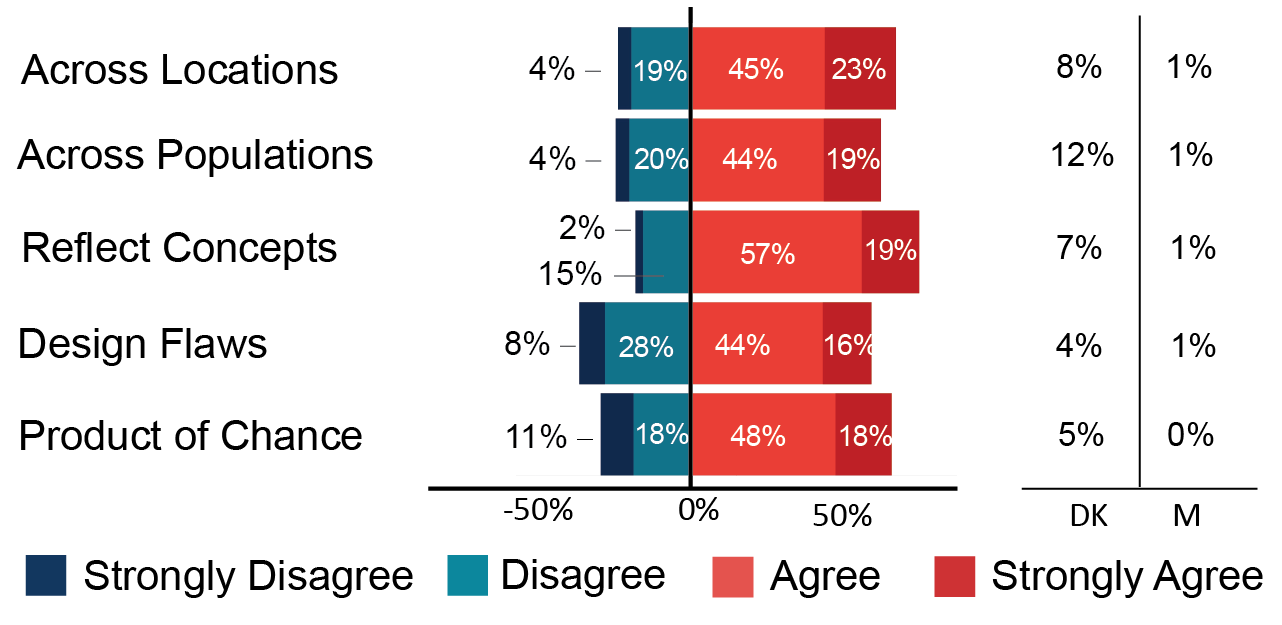
\includegraphics[scale=1]{results/figures/Fig1-Q7-Epistemology.png}
    \caption{Perceptions of the epistemological function of replication studies. Respondents identified the extent to which they agree replication studies can be used to assess the claims or features of past research; `don't know' (DK), and missing (M) responses.}
    \label{fig:Q7-Epistemology}
\end{figure}

%%%%%%%%%%%%%%%%%%%%
\newpage

\begin{figure}[hbt!]
    \centering
    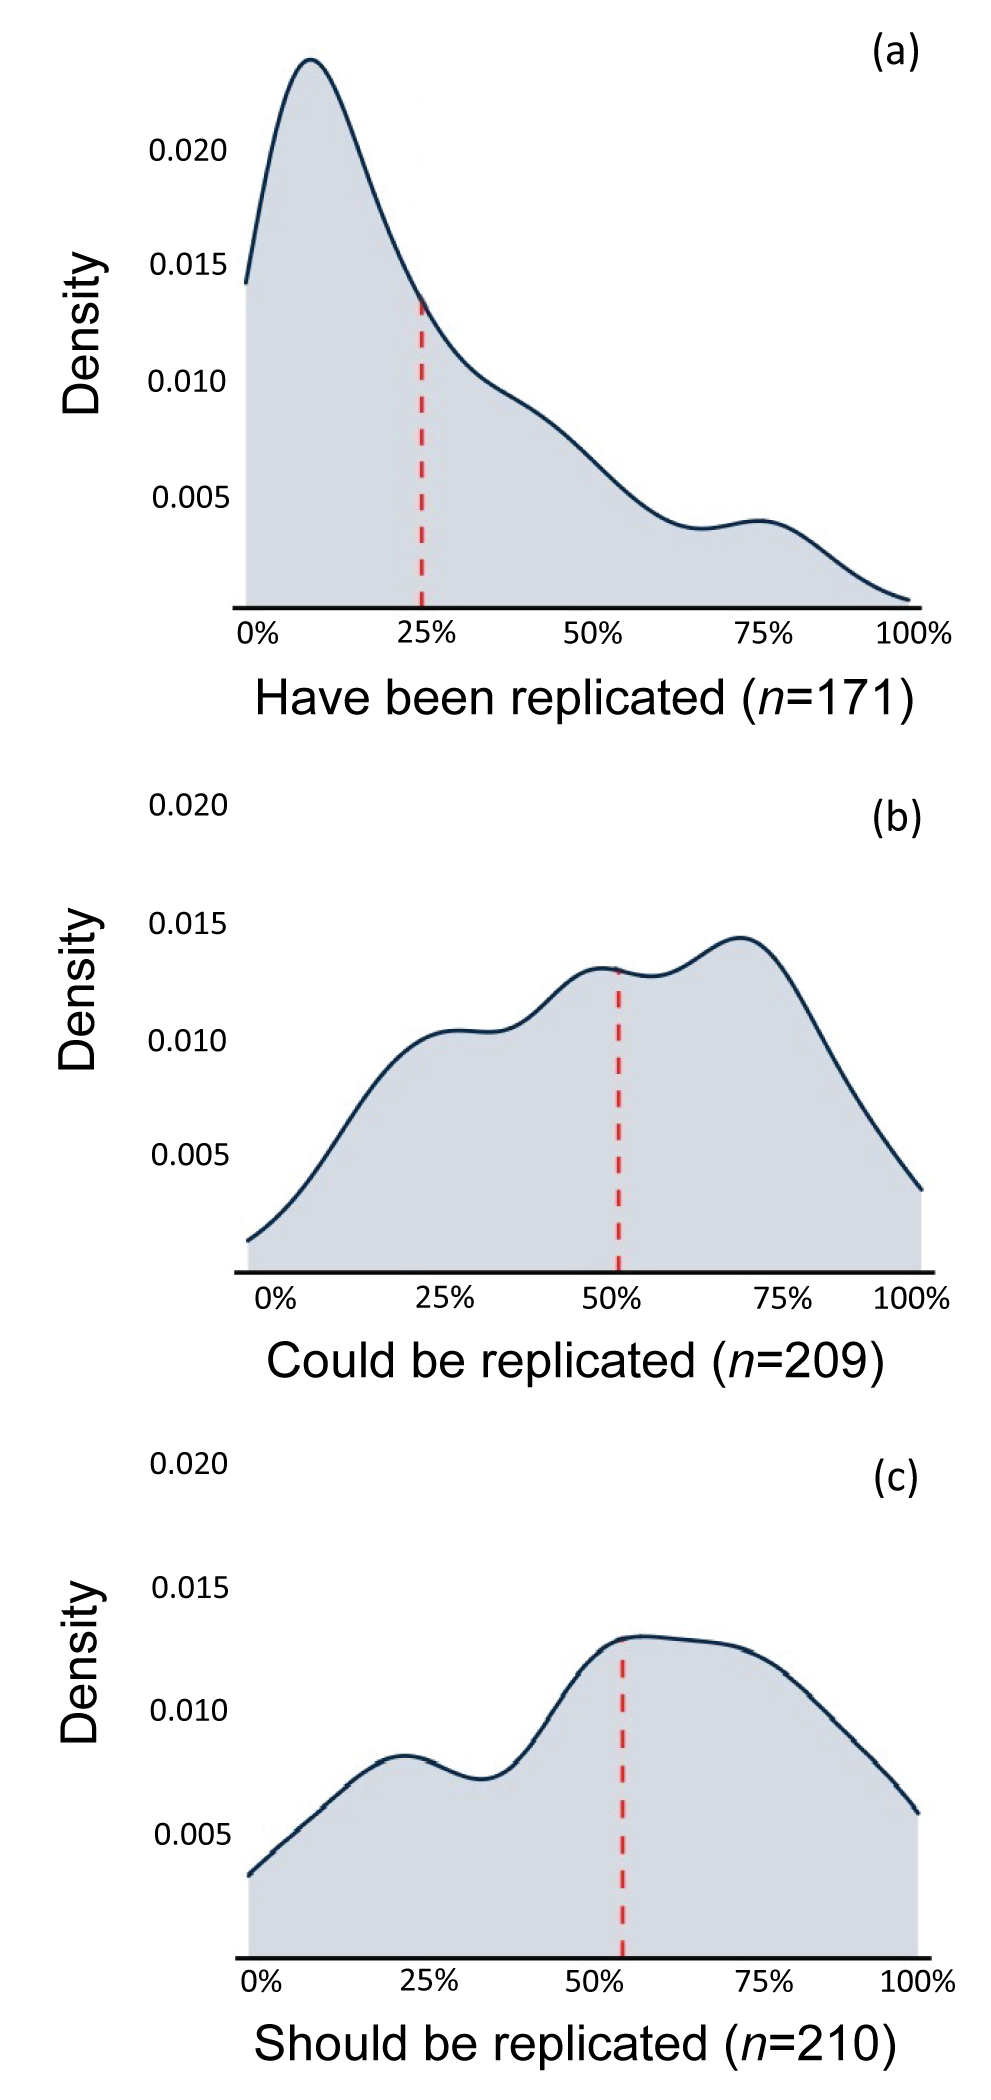
\includegraphics[scale=0.5]{results/figures/Fig2-Q12-HCS.png}
    \caption{Estimates of the percentage of geographic studies that (a) have been replicated, (b) could be replicated, or (c) should be replicated}
    \label{fig:Q12-HCS}
\end{figure}

%%%%%%%%%%%%%%%%%%%%
\newpage

\begin{figure}[hbt!]
    \centering
    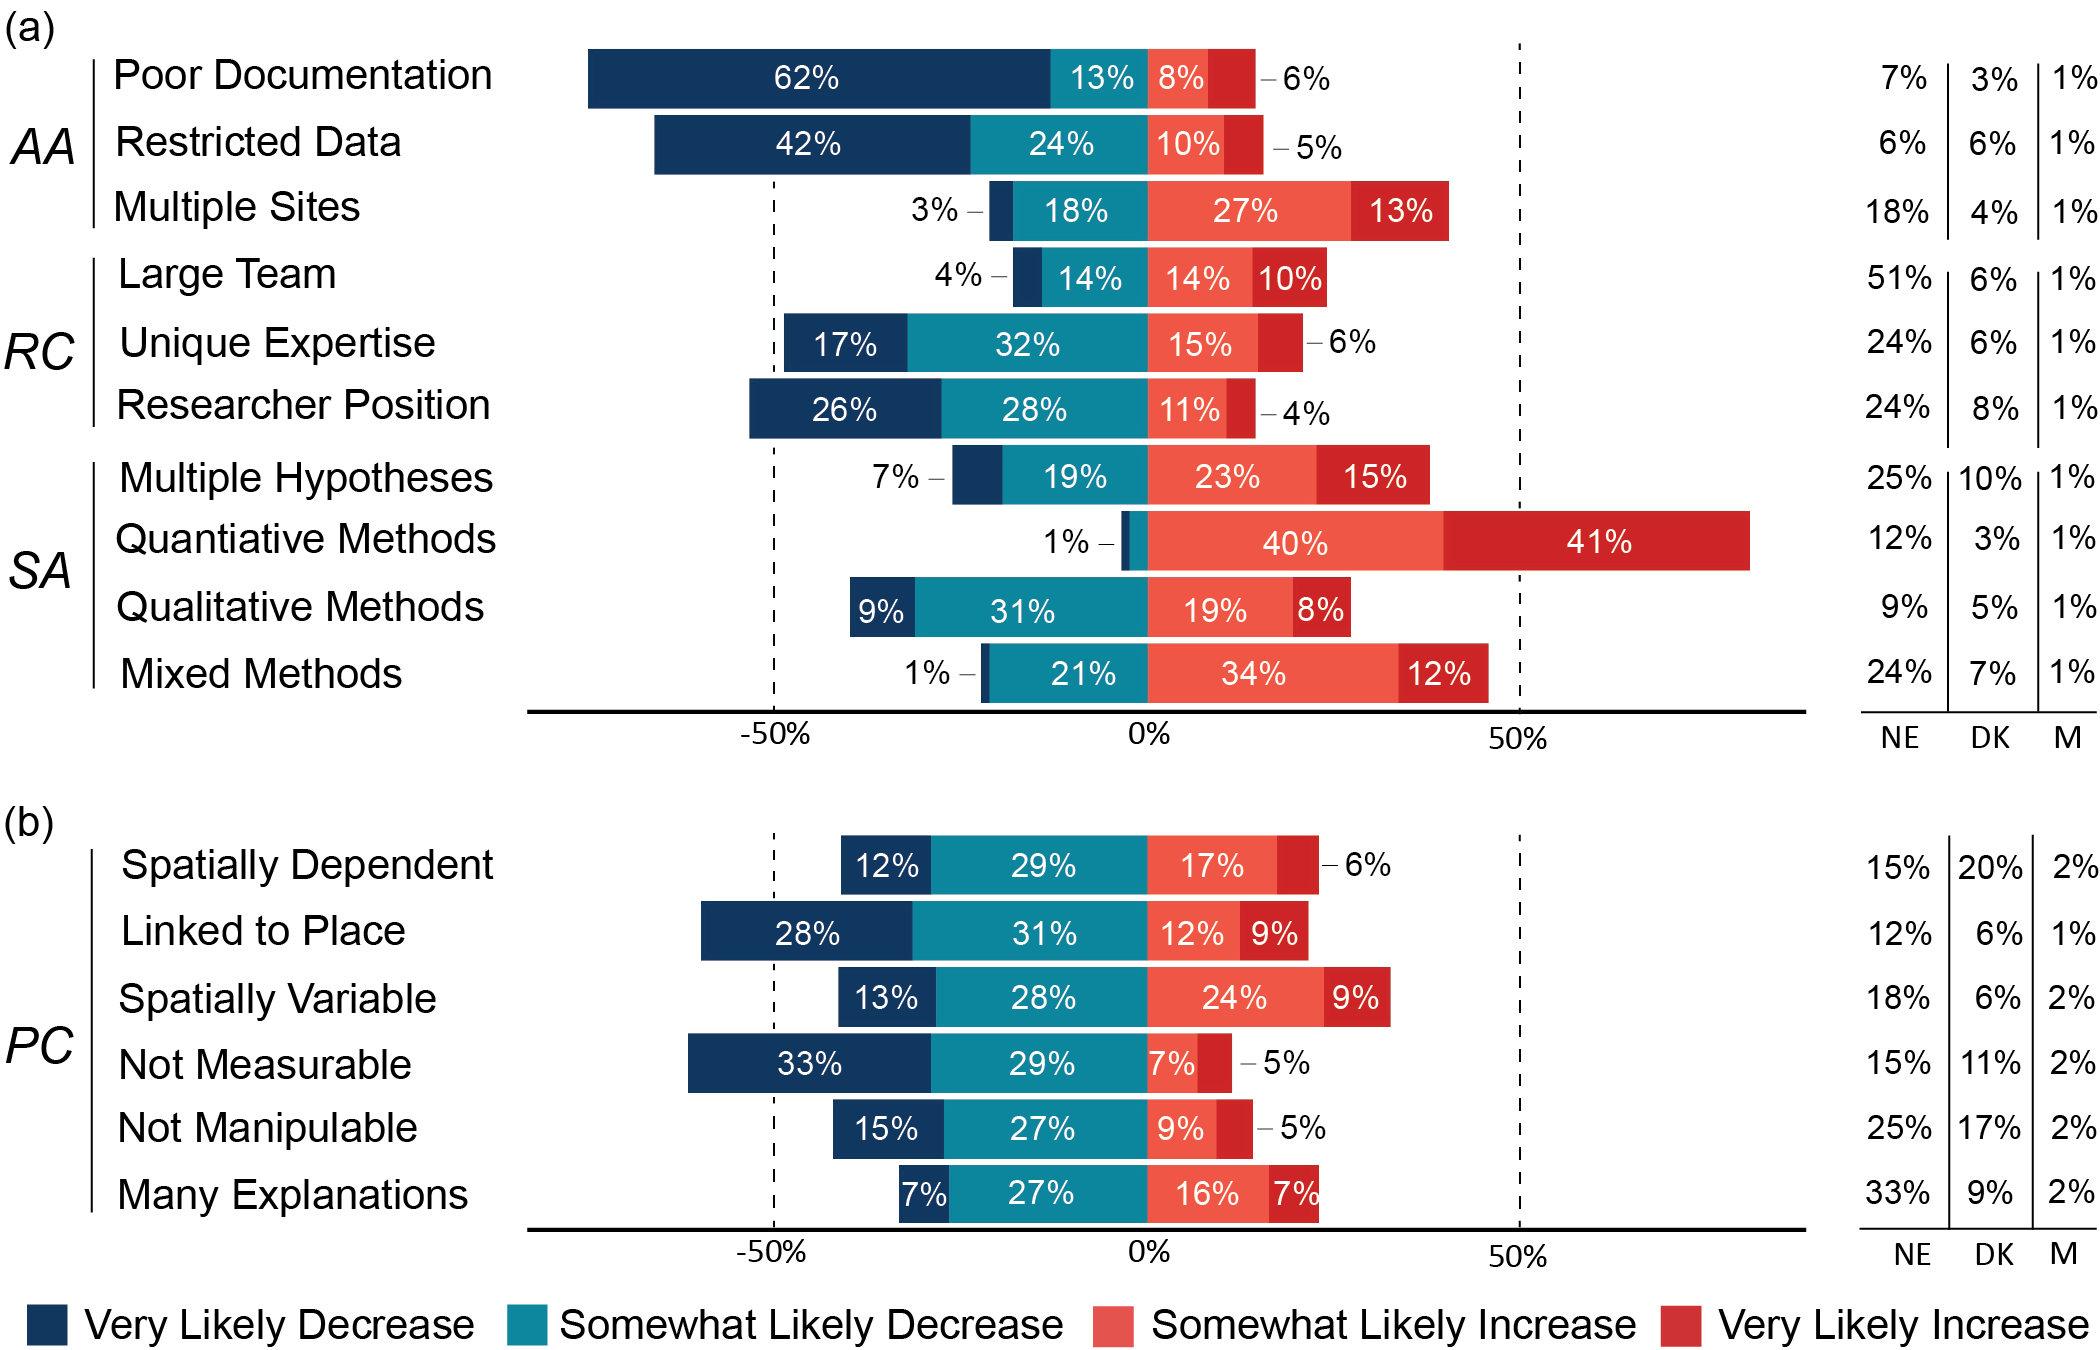
\includegraphics[scale=0.8]{results/figures/Fig3-Q8-10-Chances.png}
    \caption{Factors affecting the chances of replicating a study. Respondents identified (a) how likely study characteristics were to alter the chances of successfully replicating a study and (b) how likely the characteristics of the phenomenon under investigation were to alter the chances of successfully replicating a study in a new location. Acronyms indicate: artifact accessibility (AA), researcher characteristics (RC), study approach (SA), and phenomenon characteristics (PC); and the percentage of no effect (NE), `don't know' (DK), and missing (M) responses.}
    \label{fig:Q8-10-Chances}
\end{figure}

%%%%%%%%%%%%%%%%%%%%
\newpage

\begin{figure}[hbt!]
    \centering
    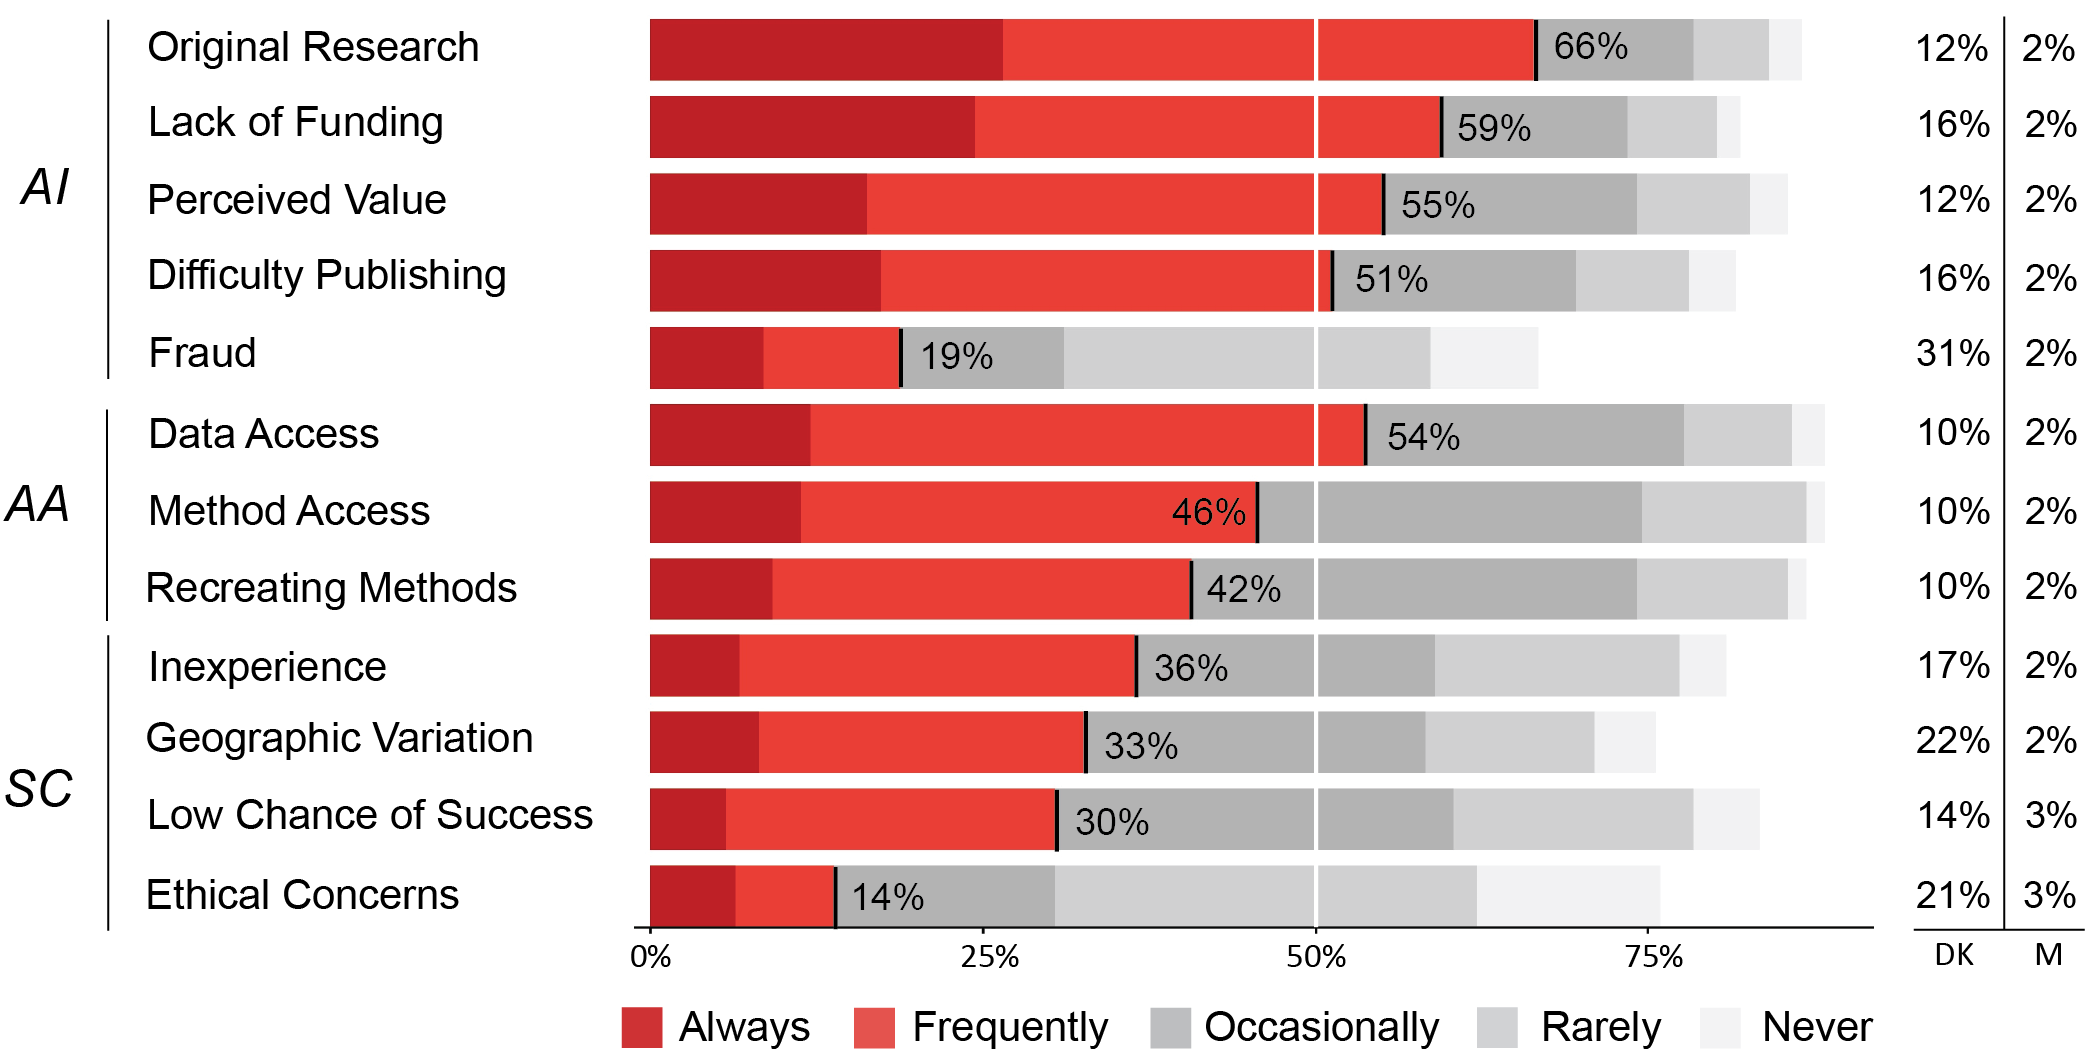
\includegraphics[scale=0.8]{results/figures/Fig4-Q15-Decisions.png}
    \caption{Factors Affecting Researcher Decisions to Undertake Replication Studies. Factors grouped by: Academic Incentives (AI), Artifact Accessibility (AA), Study Characteristics (SC); and the percentage `don't know' (DK) and missing (M) responses.}
    \label{fig:Q15-DecisionFactors}
\end{figure}

%%%%%%%%%%%%%%%%%%%%
\newpage
\noindent PETER KEDRON is an Associate Professor in Department of Geography at University of California Santa Barbara, Santa Barbara CA, 93106, US. Email: peterkedron@ucsb.edu. His research program develops and uses spatial analytical methods to understanding persistently uneven patterns of spatial development. His recent work focuses on improving the production and accumulation of knowledge used to benefit society through policy. \\  
  
\noindent JOSEPH HOLLER is an Assistant Professor of Geography at Middlebury College. He is human geographer and geographic information scientist with research interests in social vulnerability and adaptation in the context of climate change and environmental degradation. His research intersects with work in political ecology, development geography, human dimensions of global change, and geographic information science. \\
  
\noindent SARAH BARDIN is a doctoral student in Geography at the School of Geographical Sciences and Urban Planning at Arizona State University. Her research focuses on leveraging spatial modeling and GIS to generate policy-relevant, actionable insights from data.

\end{document}